\documentclass[UTF8]{ctexart}
\usepackage{bookmark}
\usepackage{geometry}
\usepackage{hyperref}
\geometry{a4paper,scale=0.8}
\usepackage{ctex}
\usepackage[style=caspervector,backend=biber,utf8]{biblatex}
\usepackage{booktabs}
\usepackage{array}
\usepackage{fancyhdr}
\pagestyle{fancy}
\fancyhf{}
\renewcommand\footrulewidth{1pt}
\lhead{王铠泽}
\rhead{PB18020766}
\chead{\href{mailto:volar@mail.ustc.edu.cn}{volar@mail.ustc.edu.cn}}
\rfoot{中国科学技术大学}
\lfoot{\today}
\usepackage{graphicx}
\usepackage{float}
\usepackage{subfigure}


\begin{document}

	\centering\textbf{\LARGE{计算物理A第八次作业}}
	
	
	王铠泽\qquad PB18020766
	
		
	\section{作业题目}
	
	\begin{itemize}
		\item 用$Monte\,\,Carlo$方法计算如下定积分,并讨论有效数字位数。
		\subitem $$I_1=\int_{0}^{2}dx\sqrt{x+\sqrt{x}}$$
		\subitem $$I_2=\int _{0}^{\frac{9}{10}}dx\int_{0}^{\frac{4}{5}}dy\int_{0}^{\frac{9}{10}}dz\int_{0}^{2}du\int_{0}^{\frac{13}{10}}dv(6-x^2-y^2-u^2-v^2) $$
	\end{itemize}
	
	\section{实现方法和原理}
	
	\begin{itemize}
		\item $Monte\,\,Carlo$简单抽样求积分
		
		单变量的情况下求$\int_{a}^{b}f(x)dx$,可以按照以下方法:
		设$\xi$为$[0,1]$上均匀随机数。则$\tilde{\xi}=(b-a)\xi+b$为$[a,b]$上的均匀随机数。抽取$\tilde{\xi}$序列(总点数为$N$),则$\langle f\rangle=\frac{1}{N}\sum_{k=1}^{N}f(\tilde{\xi})$。
		$$\Rightarrow \int_{a}^{b}f(x)dx=(b-a)\langle f\rangle=\frac{b-a}{N}\sum_{k=1}^{N}f(\tilde{\xi})$$
		
		这个结论可以推广到多变量情形:
		$$\int_{R}f(\vec{r})d\vec{r}=\langle f\rangle\cdot V(R)$$
		\begin{flushleft}
			其中$R$代表任意维度的矩形区域$[a_1,b_1]\times[a_2,b_2]\times...$,$V(R)$表示矩形区域的体积,$\langle f\rangle=\frac{1}{N}\sum_{k=1}^{N}f(\tilde{\xi})$,$\tilde{\xi}$为$R$上均匀分布的随机变量。
		\end{flushleft}
		
		\item 大数定律和中心极限定理
	
		假设$X_1,...,X_N$为服从同一分布的随机变量序列。设其期望为$\mu$,标准差为$\sigma$,$ \langle X \rangle=\frac{1}{N}\sum_{k=1}^{N}X_k$。
		大数定律指出:
		$$\frac{1}{N}(X_1+...+X_N)\stackrel{N\rightarrow\infty}{\longrightarrow}\mu$$
		中心极限定理:
		$$P(\frac{\langle X \rangle-\mu}{\sigma/\sqrt{N}}<x)\stackrel{N\rightarrow\infty}{\longrightarrow}\Phi(x)$$
		其中$\Phi(x)$为标准正态分布$\frac{1}{\sqrt{2\pi}}e^{-\frac{x^2}{2}}$。
		$$\mbox{积分结果}I=V(R)\langle f \rangle$$
		$$\mbox{积分结果方差}var(I)=V^2(R)var(\langle f \rangle)$$
		$$\mbox{积分结果标准差}\sigma(I)=V(R)\sqrt{\langle f \rangle}=V(R)\frac{\sigma(f)}{\sqrt{N}}$$
		当$N$充分大时,结果的误差是正比于$\sqrt{N}$的。
	\end{itemize}
	
	\section{程式说明}
	\begin{itemize}
		\item single.c
		
		该程式计算第一个单变量积分。
		
		\item multi.c
		
		该程式计算第二个多变量积分。
		
		\item rdm.h
			
		这是一个包含了使用16807产生器生成指定长度的$[0,1]$上均匀分布随机数函数的头文件。
		
		\subitem void rdm(int N,double *x,int method)
		
		该函数将输入的指针$x$对应的长度为$N$的数组用$[0,1]$上的随机数填满。method是关于初始种子的选择。method=0:默认种子;method=1,时间种子。程式中故意采用$sleep$函数就是为了得到不同的时间种子。
		
		\item time\_seed\_single/multi.txt
		
		16807产生器抽样时对应的时间种子数据(1个种子)。调用多少次16807生成器就生成多少个数据记录。
		
		\item single\_variable/multi\_variable.txt
		
		详细记录了不同$N$下的积分值$I$以及其和准确值之间的误差$Err$。
	\end{itemize}
	
	\section{计算结果}
	
	\subsection{单变量积分}
	
	\begin{flushleft}
		对于积分:
	\end{flushleft}
	 $$I_1=\int_{0}^{2}dx\sqrt{x+\sqrt{x}}$$
	使用$Mathematica$得到其准确值约为$I\approx2.689521304816752$。
	不同$N$下对应的情况如下表所示。

		\begin{table}[H]
		\centering
		\setlength{\tabcolsep}{10mm}{
			\begin{tabular}{@{}llll@{}}
				\toprule
				$N$&$Integral$&$Error$&$\frac{1}{\sqrt{N}}$\\ \midrule
				$ 10 $	&2.29035867e+000	&3.99162639e-001	&3.16227766e-001\\
				$ 10^2 $	&2.64702903e+000	&4.24922760e-002	&1.00000000e-001\\
				$ 10^3 $	&2.71176247e+000	&2.22411622e-002	&3.16227766e-002\\
				$ 10^4 $	&2.67987859e+000	&9.64271888e-003	&1.00000000e-002\\
				$ 10^5 $	&2.68859115e+000	&9.30158296e-004	&3.16227766e-003\\
				$ 10^6 $	&2.68942442e+000&\textbf{	9.68839664e-005	}&\textbf{1.00000000e-003}\\
				$ 10^7 $	&2.68944262e+000	&7.86839022e-005&	3.16227766e-004\\
				$ 10^8 $	&2.68942564e+000	&9.56666747e-005&	1.00000000e-004\\
				
				\bottomrule
		\end{tabular}}
		\caption{不同$N$下单变量积分的情况(采用科学计数法)}
	\end{table}

	\begin{center}
		\textbf{
			可见,当$N$越来越大时,标准差和$\frac{1}{\sqrt{N}}$逐渐接近。}
	\end{center}

		\subsection{多变量积分}
	
	\begin{flushleft}
		对于积分:
	\end{flushleft}
$$I_2=\int _{0}^{\frac{9}{10}}dx\int_{0}^{\frac{4}{5}}dy\int_{0}^{\frac{9}{10}}dz\int_{0}^{2}du\int_{0}^{\frac{13}{10}}dv(6-x^2-y^2-u^2-v^2) $$
	使用$Mathematica$得到其准确值约为$I\approx5.644079999999997$。
	不同$N$下对应的情况如下表所示。
	
	\begin{table}[H]
		\centering
		\setlength{\tabcolsep}{10mm}{
			\begin{tabular}{@{}llll@{}}
				\toprule
				$N$&$Integral$&$Error$&$\frac{1}{\sqrt{N}}$\\ \midrule
			
				$ 10 $		&6.17363991e+000	&5.29559909e-001	&3.16227766e-001\\
				$ 10^2 $	&5.14681851e+000	&4.97261489e-001	&1.00000000e-001\\
				$ 10^3 $	&5.69498165e+000	&5.09016489e-002	&3.16227766e-002\\
				$ 10^4 $	&5.67040355e+000	&2.63235535e-002	&1.00000000e-002\\
				$ 10^5 $	&5.64101095e+000	&3.06904571e-003	&3.16227766e-003\\
				$ 10^6 $	&5.64586026e+000	&1.78026028e-003	&1.00000000e-003\\
				$ 10^7 $	&5.64415403e+000	&7.40250527e-005	&3.16227766e-004\\
				\bottomrule
		\end{tabular}}
		\caption{不同$N$下多变量积分的情况(采用科学计数法)}
	\end{table}
	
	\begin{center}
		\textbf{
			可见,当$N$越来越大时,标准差和$\frac{1}{\sqrt{N}}$逐渐接近。}
	\end{center}

	\subsection{误差分析}
	对单变量情况,做出对数$Error-1/\sqrt{N}$拟合曲线如下:
	
		\begin{figure}[H]
		\centering  %图片全局居中
		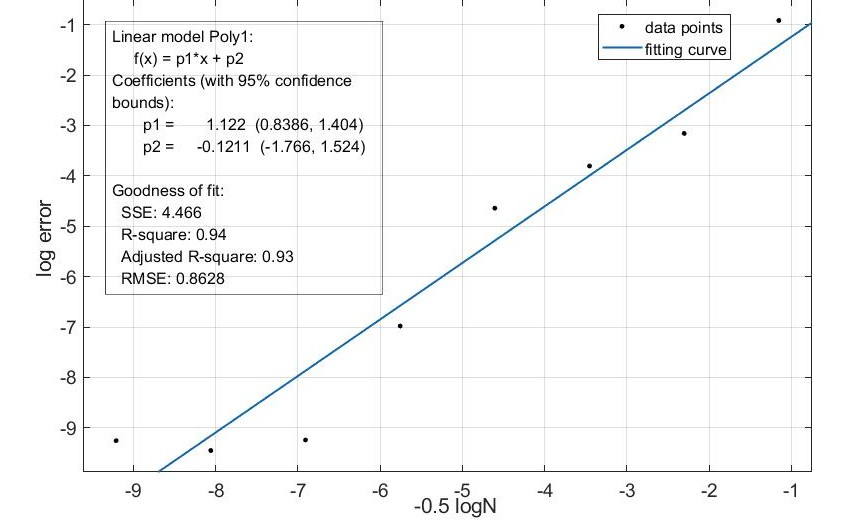
\includegraphics[width=6in]{../figure/single.jpg}
		\caption{单变量积分$log(\epsilon)-log(\frac{1}{\sqrt{N}})$}
	\end{figure}
	
	对多变量情况,做出对数$Error-1/\sqrt{N}$拟合曲线如下:
	\begin{figure}[H]
		\centering  %图片全局居中
		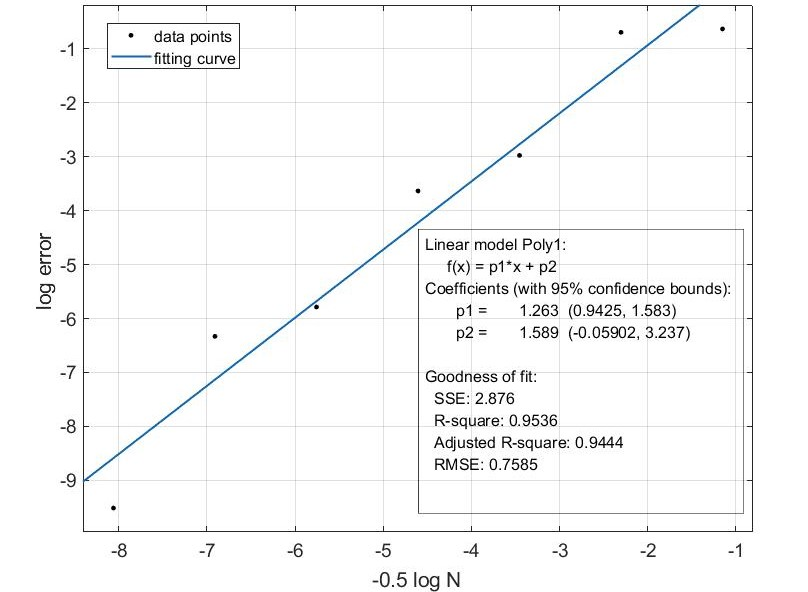
\includegraphics[width=6in]{../figure/multi.jpg}
		\caption{多变量积分$log(\epsilon)-log(\frac{1}{\sqrt{N}})$}
	\end{figure}

	\textbf{拟合结果可以看出误差$\epsilon\sim1/\sqrt{N}$}
	\section{总结}
	\begin{itemize}
		\item 本次实验使用$Monte\,\,Carlo$方法求简单区间上的积分值,在$N$较大的时候很接近准确值。
		\item 随着对精确度$\epsilon$要求提高,对抽样点数$N$的增长大约是是小数点后每精确一位就需要增长100倍,高精度计算只用简单抽样的$Mone\,\,Carlo$方法显然是不实际的,需要其他的优化。
		\item 由于点数有限和生成随机数的初始种子,生成方式等影响,误差并不严格满足中心极限定理预言的$\frac{1}{\sqrt{N}}$,有时甚至会略小(见前述的单变量实验表格)。
	\end{itemize}
	\clearpage
\end{document}